\label{afgraensning}
\subsection{Valg af fokusområde}
I vores problemanalyse har vi kigget på de teknologiske og samfundsmæssige problemer omkring teknologien. Der har været problemer af begge typer, men de problemer som har vist sig i form af ulykker for bilen, har været fordi bilen ikke har kørt som andre mennesker. Som nævnt i afsnit \ref{interaktion}, kører den selvkørende bil blandt andet ikke aggressivt nok, hvilket har forårsaget at biler er kørt op bag i den.

\subsection{Bilens syn}
Så hvordan undersøger bilen hvad der er rundt om den? Både Tesla og Audi benytter sig af Nvidia Drive PX, hvilket er en udviklingsplatform, som tillader bilen det er installeret i, at tilgå Nvidias nye deep-learning platform kaldet DIGITS. Dette gør det muligt for enheder, at lære deres omgivelser at kende, og er designet til at fungere ligesom et menneske. 

\begin{figure}[h!]
	\centering
	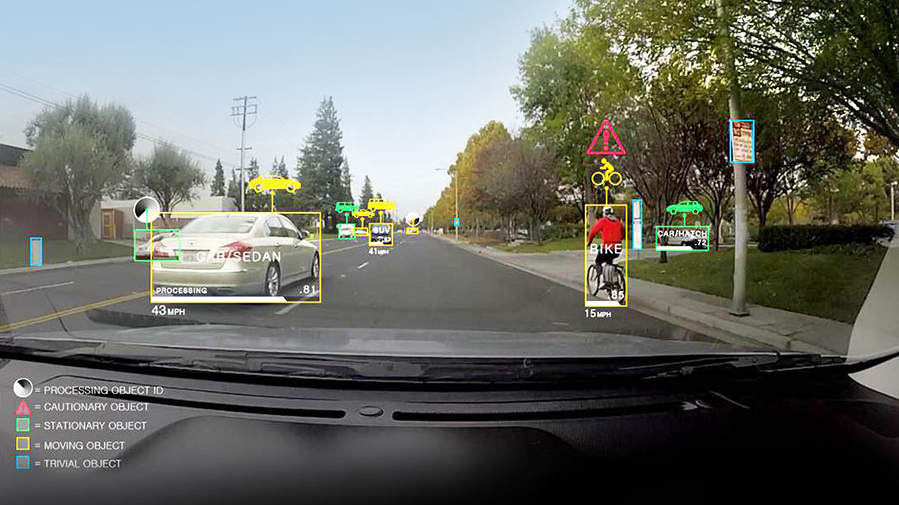
\includegraphics[width=\textwidth]{images/nvidiadrive.png}
	\captionsource{Nvidia DRIVE PX analyserer omgivelserne, og kan inddele objekter i forskellige grupper.}{\url{https://www.nvidia.com/object/drive-px.html}}
	\label{fig:DRIVE}
\end{figure}
Ligesom mennesker lærer med tiden og af deres erfaringer, vil bilerne også lære af deres erfaringer, men da de alle er koblet til dette netværk, lærer alle bilerne, af alle bilers erfaringer \cite{Nvidia}. Dette board uploader sine data til DIGITS, og hvis der er noget indsamlet data den ikke er sikker på hvad den skal gøre med, vil dette data blive kigget og regnet på af hele netværket.

DIGITS analyserer billeder fra kamerarer rundt om bilen, og inddeler objekterne rundt om bilen i klasser. På figur \ref{fig:DRIVE} kan man se hvordan objekter er klassificeret på et stilbillede.

DIGITS er selvfølgelig kun \'en platform, og andre producenter af selvkørende biler vil måske benytte sig af andre systemer. Men det vigtigste er blot at kunne skille de forskellige objekter fra hinanden \cite{cnet}, så ikke alt ses som den samme type objekter. Grunden til dette er, at bilen skal kunne forholde sig anderledes over for en cyklist, end for en anden bil. Programmet bliver nødt til at kende forskellen på en parkeret bil der holder i vejkanten, og en bil som kommer fra en sidevej og kan finde på at køre ud foran den selvkørende bil. Normaltvist vil et menneske forsøge at få øjenkontakt med en billist som kommer fra en sidevej, for at sikre sig at bilen er blevet set, men da en selvkørende bil ikke kan lave øjenkontakt, bliver den nødt til at kunne adskille de forskellige typer af objekter på vejene.

\subsection{Typer af trafikanter}
Det er vigtigt at en selvkørende bil kan adskille forskellige typer af trafikanter, da de hver især har forskellige karakteristika. I en rapport fra Havarikommissionen for vejtrafikulykker viser resultaterne, at størstedelen af de ulykker der skete mellem cyklister og billister skyldtes dårlige trafikvaner \cite{HVU}. I 17 ud af 30 undersøgte ulykker havde cyklisten vigepligt, men kørte alligevel ud i krydset. Undersøgelsen konkluderer at både cyklister og billister var opmærksomme, og at ulykkerne overvejende skyldtes dårlige trafikvaner. 

Hvad betyder det så for de selvkørende biler? Det betyder at hvis bilen opdager en cyklist, bliver den nødt til at vide at nogle cyklister har dårlige trafikvaner, og at den derfor skal være opmærksom på at cyklisten ikke nødvendigvis vil køre efter de gældende trafikregler. 

For motorcykler er det dog et andet problem der skal tages hensyn til.  I en undersøgelse fra Havarikommisionen offentliggøres det at ud af 41 ulykker vedrørende motorcykler, kunne halvdelen af ulykkerne være undgået hvis motorcyklisten havde haft en mere moderat hastighed \cite{MOT}. For den selvkørende bil kan dette også have en betydning, hvor den skal til at tænke over om motorcyklister har for høj en fart, og hvordan den skal reagere i forhold til en eventuel forhøjet fart.

I forhold til billister har vi allerede i afsnit \ref{interaktion} set på eksempler, hvor folk er kørt ind i Googles selvkørende bil, fordi den er bremset op til et gult lys. Bilen skal derfor være i stand til forudsige om bilen bagved vil stoppe. For hvis den selvkørende bil kan nå over lyskrydset inden det bliver rødt, vil dette være at foretrække frem for at være i fare for at bilen bagved påkører den selvkørende bil.

Til sidst har vi så fodgængerne, som skal tages hensyn til. Bilen skal kunne kende forskel på en voksen og et barn, da der skal køres mere forsigtigt omkring børn. Fodgængere skal altså kunne klassificeres i forhold til hvor ``uberegnelige'' de er. 